\documentclass{article}
\usepackage{amsmath}
\usepackage{amssymb}
\usepackage[usenames, dvipsnames]{color}
\usepackage{fancyhdr}
\usepackage{hyperref}
\usepackage{tikz}
\usepackage{geometry}

\geometry{letterpaper, portrait, margin=0.5in}
\pagestyle{fancy}

\fancyhf{} % clear all header fields
\renewcommand{\headrulewidth}{0pt}
\fancyfoot[LE,RO]{\thepage}           % page number in "outer" position of footer line
\fancyfoot[RE,LO]{\copyright\;aquarc 2025. \href{https://aquarc.org}{\underline{aquarc.org}}} % other info in "inner" position of footer line

\definecolor{myred1}{RGB}{255, 0, 0}
\definecolor{myyellow1}{RGB}{255, 255, 219}
\definecolor{mygreen1}{RGB}{0, 255, 0}
\definecolor{mygreen2}{RGB}{0, 126, 0}
\definecolor{myblue1}{RGB}{0, 0, 255}

\begin{document}

\fontsize{14}{16}\selectfont

% center the title
\begin{center}
    \textbf{\underline{Sets Cheatsheet}}
\end{center}

\tableofcontents
\pagebreak

\section{Geometric Series}
Geometric Series are a special type of Power Series that can be rewritten in the form

$$
f(x)=\frac{a_1}{1-r}=\sum_{n=0}^{\infty}{
    a_1*r^n
}
$$

\subsection{Proof}
\begin{align*}
    S=a_1+a_1r+a_1r^2+a_1r^3+...+a_1r^n+... \\
    rS=a_1r+a_1r^2+a_1r^3+a_1r^4...+a_1r^n+... \\
    S-rS=a_1+a_1r-a_1r+a_1r^2-a_1r^2+...+a_1r^n-a_1r^n+a_1r^{n+1}+... \\
    \Longrightarrow S(1-r)=a_1+a_1r^{n+1}
\end{align*}
Evaluate the $\lim$ as $n \to \infty$

\begin{align*}
    S=\lim_{n \to \infty}{\frac{a_1+a_1r^{n+1}}{1-r}}
\end{align*}

We can only evaluate this equation when $|r|<1$. Therefore:
$$
\frac{a_1}{1-r}
$$
Is the sum of the geometric series.

To find the interval of convergence, just remember that $|r|< 1$

\subsection{Examples}
$$
f(x)=\frac{1}{2-x}, c=0 
\Longrightarrow f(x)=\frac{1}{2}*\frac{1}{1-\frac{x}{2}}
\Longrightarrow f(x)=\sum_{n=0}^{\infty}{\frac{1}{2}*(\frac{x}{2})^n}
$$
$$
\Longrightarrow f(x)=\sum_{n=0}^{\infty}{(\frac{1}{2})^{n+1}x^n}
$$
$$
|r|<1 
\Longrightarrow |\frac{x}{2}|<1
\Longrightarrow |x|<2
\Longrightarrow x \in (-2,2)
$$

If we change the center:
$$
f(x)=\frac{1}{2-x}, c=5 \Longrightarrow f(x)=\frac{1}{2-5-(x-5)} 
\Longrightarrow \frac{1}{-3-(x-5)}
$$
$$
\Longrightarrow -\frac{1}{3}*\frac{1}{1-\frac{-(x-5)}{3}}
\Longrightarrow \sum_{n=0}^{\infty}{-\frac{1}{3}*(\frac{-(x-5)}{3})^n}
$$
$$
\Longrightarrow \sum_{n=0}^{\infty}{(-\frac{1}{3})^{n+1}(-(x-5))^n}
$$
$$
|r|<1
\Longrightarrow r \in (-1,1)
\Longrightarrow \frac{-x+5}{3} \in (-1,1)
\Longrightarrow -(x-5) \in (-3,3)
\Longrightarrow x \in (2,8)
$$
 
Now let's completely change it up.

$$
f(x)=\frac{3}{2x-1}, c=0 
\Longrightarrow f(x)=-3*\frac{1}{1-2x}
\Longrightarrow *\sum_{n=0}^{\infty}{-3*(2x)^n}, c \in (-\frac{1}{2},\frac{1}{2})
$$
Let's move the center
$$
f(x)=\frac{3}{2x-1}, c=-3
\Longrightarrow f(x)=\frac{1}{2(x+3)-5-6}
\Longrightarrow f(x)=-\frac{1}{11}*\frac{1}{1-\frac{2}{11}(x+3)}
$$
$$
f(x)=\sum_{n=0}^{\infty}{-\frac{1}{11}*(\frac{2}{11}(x+3))^n}
$$
$$
\frac{2}{11}(x+3) \in (-1,1) 
\Longrightarrow (x+3) \in (-\frac{11}{2},\frac{11}{2}) 
\Longrightarrow x \in (-\frac{17}{2},\frac{5}{2})
$$

What if there is no $-x$? You can just do $-(-x)$. Remember: Basic Algebra will take you a long way.

$$
f(x)=\frac{3}{x+2}, c=0 \Longrightarrow f(x)=\frac{3}{2}*\frac{1}{1-\frac{1}{2}(-x)}
$$

What if your function looks a bit more complicated?
$$
f(x)=\frac{4x-7}{2x^2+3x-2}, c=0
\Longrightarrow f(x)=\frac{4x-7}{(2x-1)(x+2)}
\Longrightarrow f(x)=\frac{A}{2x-1}+\frac{B}{x+2}
$$
$$
A(x+2)+B(2x-1)=4x-7 
\Longrightarrow Ax+2Bx=4x, 2A-B=-7
\Longrightarrow B=2A+7 
$$
$$
\Longrightarrow A+4A+14=4 
\Longrightarrow 5A=-10 
\Longrightarrow A=-2, B=3
$$
$$
f(x)=\frac{-2}{2x-1}+\frac{3}{x+2}
$$
Solve it normally from here.

\section{General Power Series}
$$
f(x)=\sum_{n=0}^{\infty}{\frac{f^{(n)}(c)}{n!}(x-c)^n}
$$

\subsection{Derivation}
We take general power series to be something like the following:
$$
f(x)=1+x+2x^2+3x^3+...+nx^n+...
$$
or
$$
f(x)=1+x+\frac{1}{2}x^2+\frac{1}{3}x^3+...+\frac{1}{n}x^n+...
$$

So generally:
$$
f(x)=\sum_{n=0}^{\infty}{a_n(x-c)^n}
$$
Instead of $a_i$ because the coefficient changes for each element in the series. Let's expand this series:

$$
f(x)=a_0+c+a_1(x-c)+a_2(x-c)^2+a_3(x-c)^3+...+a_n(x-c)^n + ...
$$
Take its derivative:
$$
f'(x)=0+a_1+2a_2(x-c)+3a_3(x-c)^2+...+na_n(x-c)^{n-1}+...
$$
Notice how $f'(0)=a_1$.
$$
f''(x)=0+0+2a_2+6a_3(x-c)+...+n(n-1)a_n(x-c)^{n-2}+...
$$
Notice how $f''(0)=2a_2$ and $f'''(0)=6a_3$. In order to get the $a_n$ term, you just need to take $f^{(n)}(c)$ and divide it by $n!$ \\
Put it together, and you'll get the equation we started with.

\subsection{Examples}
$$
f(x)=e^x,c=0
\Longrightarrow f(x)=\sum_{n=0}^{\infty}{\frac{e^0}{n!}(x)^n}
\Longrightarrow f(x)=\sum_{n=0}^{\infty}{\frac{x^n}{n!}}
$$
$$
\Longrightarrow 1+x+\frac{1}{2}x^2+\frac{1}{3}x^3+...+\frac{1}{n}x^n+...
$$
Evaluate a geometric series using Taylor series
$$
f(x)=\frac{1}{1-2x},c=0
\Longrightarrow \frac{\frac{1}{1-2(0)}}{0!}+
\frac{\frac{2}{(1-2c)^2}}{1!}x +
\frac{\frac{8}{(1-2c)^3}}{2!}x +
\frac{\frac{48}{(1-2c)^4}}{3!}x+...
$$
$$
\Longrightarrow 1+\frac{2}{(1-2c)^2}x+\frac{4}{(1-2c)^3}x^2+\frac{8}{(1-2c)^4}x^3+...
$$
General term: $2^nx^n$. \\

We would have gotten the same thing if we used the power series expansion of the Taylor series expansion. As with most things in algebra, pick the method that's \textbf{most conveinient for you}.

\subsection{Error Checking}
In an ideal world, you want to know how far off your estimates are. For alternating series, this process is pretty easy.

$$
f(x)=1-x+\frac{x}{2!}-\frac{x}{3!}+\frac{x}{4!}-\frac{x}{5!}+\frac{x}{6!}-\frac{1}{7!}+...+\frac{1}{n!}(-1)^n+...
$$
Let's choose the first four terms for our \textbf{Taylor Polynomial}, which will be represented by $P_n(x)$ where $n$ is the degree.
$$
P_4(x)=1-x+\frac{1}{2}x^2-\frac{1}{3}x^3
$$
Let's set the remainder terms to $R_5(x)$. We can call the error $E(x)$.

$$
E(x)=|P_4(x)-R_5(x)|
$$

Since you will never truly know $R_5(x)$ or any $R_n(x)$ for that matter, you will never know the true error. But you can set an upper bound on that error, which is pretty easy in alternating power series.\\

$$
E(x)\leq P_{n+1}(x) - P_{n}(x)
$$
A fancy way of saying, the term right after is the highest the eror can be. It's because you will never add back what you subtracted, always less.

\subsection{Deriving $e^a$}
We can use a Taylor Series to derive $e^a$!
\begin{align*}
    \lim_{n \to \infty}{(1+\frac{a}{n})^n}=L
    \Longrightarrow \ln(\lim_{n \to \infty}{(1+\frac{a}{n})^n})=\ln L
    \Longrightarrow n\ln(\lim_{n \to \infty}{(1+\frac{a}{n})})=\ln L \\
    t=\frac{a}{n}, \Longrightarrow \frac{a}{t}(\lim_{n \to \infty}{\ln(1+t)})=\ln L
    \Longrightarrow \frac{a}{t}(\lim_{t \to 0}{\ln(1+t)})=\ln L \\
    \longrightarrow \ln(1+t)=t-\frac{t^2}{2}+\frac{t^3}{3}+...\approx t \\
    \Longrightarrow \ln L=a \Longrightarrow L=e^a
\end{align*}

\subsection{Lagrange Error Checking}
If your series \textbf{isn't alternating}, you can use Lagrange Error Checking. Although the proof is complicated, it's pretty simple
$$
E(x)\leq|\frac{\max_{z \in [x,c]}{f^{(n+1)}(z)}}{(n+1)!}|(x-c)^{n+1}
$$

The proof isn't necessary for Calc BC. You can find it online. 
\subsubsection{Full Example}
Find the first four terms about $c=2$ for $ln|x+1|$. 

We can start with its derivative, $\frac{1}{x+1}$.\\
For simplicity, we will use a geometric series.
Say we wanted to find $\ln|\frac{3}{2}|$ and approximate error to be 0.05 or less

\begin{align*}
    \frac{1}{x-1}=\frac{1}{1-(x-2)+2}=\frac{1}{-1-(x-2)}=-\frac{1}{1-(-(x-2))} \\
    \Longrightarrow \sum_{n=0}^{\infty}{-(-(x-2))^n} = 
    \sum_{n=0}^{\infty}{(-1)^{n+1}(x-2)^n} = -1+(x-2)-\frac{1}{2}(x-2)^2+\frac{1}{3}(x-2)^3+... \\
    \int{-\frac{1}{1-(-(x-2))}}dx = \int{-1+(x-2)-\frac{1}{2}(x-2)^2+\frac{1}{3!}(x-2)^3+...}dx \\
    \Longrightarrow -\ln|1-(-(x-2))|=C-x+\frac{(x-2)^2}{2}-\frac{(x-2)^3}{3*2!}+\frac{(x-2)^4}{4*3!}+... \\
    \longrightarrow \ln|1-(-(2-2))|=\ln|1| \\
    \longrightarrow C+x-\frac{(x-2)^2}{2}+\frac{(x-2)^3}{3*2!}-\frac{(x-2)^4}{4*3!}+... \\
    \longrightarrow \ln|1|=C+2+0+... \longrightarrow C=-2 \\
    \Longrightarrow \ln|1-(-(x-2))|=-2+x-\frac{(x-2)^2}{2}+\frac{(x-2)^3}{3*2!}-\frac{(x-2)^4}{4*3!}+... \\
    \Longrightarrow \ln|\frac{3}{2}|=\ln|1-(-(\frac{5}{2}-2))|=
    (\frac{5}{2}-2)-\frac{(\frac{5}{2}-2)^2}{2}
    +\frac{(\frac{5}{2}-2)^3}{3*2!}-\frac{(\frac{5}{2}-2)^4}{4*3!}+...\\
    \Longrightarrow  \frac{1}{2}-\frac{1}{2}*(\frac{1}{2})^2+\frac{1}{3}*(\frac{1}{2})^3
    -\frac{1}{4}*(\frac{1}{2})^4+...\\
\end{align*}
Since it's an alternating series, it should be pretty simple to solve for from here.
\subsubsection{Another Problem}
$$
\sin(5x+\frac{\pi}{4})=\sin(5(x+\frac{\pi}{20}))
$$
% yeah i'm not doing this lol

\section{Convergent or Divergent}

\subsection{Divergence Test}
If
$$
\lim_{x \to \infty}f(x)\neq 0
$$
then $f$ is divergent. If
$$
\lim_{x \to \infty}f(x)=0
$$
then use another test, it's inconclusive.

\subsection{Ratio Test}

Commonly used for geometric series, if you just check to make sure $|r|<1$ then it's going to converge. 

$$
\lim_{n \to \infty}{|\frac{a^{n+1}}{a^n}|}
$$

Basically checking that for some far off value, the common ratio remains. \\
Example:

\begin{align*}
    \sum_{n=0}^{\infty}{\frac{(-1)^{n-1}n^2}{2^n}}
    \Longrightarrow \lim_{n \to \infty}{|\frac{\frac{(-1)^{n}(n+1)^2}{2^{n+1}}}
        {\frac{(-1)^{n-1}n^2}{2^n}}|}=0
    \Longrightarrow \lim_{n \to \infty}{|\frac{(-1)^{n}(n+1)^2*2^n}{2^n*2*(-1)^{n-1}n^2}|} \\
    \Longrightarrow \lim_{n \to \infty}{|\frac{(n+1)^2}{2*-1*n^2}|}=\frac{1}{2}
\end{align*}

If $|r|=1$, we have a problem. Recall the limit from the geometric series proof:
$$
\lim_{n \to \infty}{\frac{a-ar^{n+1}}{1-r}}
$$

That's going to be undefined. So we have to use another test.

\subsubsection{More Examples}

\begin{align*}
    \sum_{n=0}^{\infty}{\frac{e^n}{n^3}}
    \Longrightarrow \lim_{n \to \infty}{|\frac{\frac{e^n*e}{(n+1)^3}}{\frac{e^n}{n^3}}|}
    \Longrightarrow \lim_{n \to \infty}{|\frac{e*n^3}{(n+1)^3}|}=e\not < 1
\end{align*}
Divergent
\begin{align*}
    \sum_{n=0}^{\infty}{\frac{(n!)^2}{(3n)!}}
    \Longrightarrow \lim_{n \to \infty}{|\frac{\frac{((n+1)!)^2}{(3n+3)!}}{\frac{(n!)^2}{(3n)!}}|}
    \Longrightarrow \lim_{n \to \infty}{|\frac{((n+1)!)^2*(3n)!}{(3n+3)!*(n!)^2}|} \\
    \Longrightarrow \lim_{n \to \infty}{|\frac{(n+1)^2*(n!)^2*(3n)!}{(3n+3)*(3n+2)*(3n+1)*(3n)!*(n!)^2}|} \\
    \Longrightarrow \lim_{n \to \infty}{|\frac{(n+1)^2}{(3n+3)*(3n+2)*(3n+1)}|}=0<1
\end{align*}
Convergent
\begin{align*}
    \sum_{n=0}^{\infty}{\frac{n!}{n^{n+1}}}
    \Longrightarrow \lim_{n \to \infty}{|\frac{\frac{(n+1)!}{(n+1)^{n+2}}}{\frac{n!}{n^{n+1}}}|}
    \Longrightarrow \lim_{n \to \infty}{|\frac{(n+1)!*n^{n+1}}{n!*(n+1)^{n+2}}|}
    \Longrightarrow \lim_{n \to \infty}{|\frac{n!*n^{n+1}}{n!*(n+1)^{n+1}}|} \\
    \Longrightarrow \lim_{n \to \infty}{|(\frac{n}{n+1})^{n+1}|}=
                    \lim_{n \to \infty}{|(\frac{n+1-1}{n+1})^{n+1}|}=
                    \lim_{n \to \infty}{|(1-\frac{1}{n+1})^{n+1}|}=\\
                    \lim_{n \to \infty}{|(1+\frac{(-1)}{n+1})^{n+1}|}=e^{-1}<1
\end{align*}
Convergent
\begin{align*}
    \sum_{n=1}^{\infty}{\frac{3^{1-2n}}{n^2+1}}
    \Longrightarrow \lim_{n \to \infty}{|\frac{\frac{3^{1-2n-2}}{(n+1)^2+1}}{\frac{3^{1-2n}}{n^2+1}}|}
    \Longrightarrow \lim_{n \to \infty}{|\frac{3^{-1-2n}*(n^2+1)}{(n+1)^2+1*3^{1-2n}}|} \\
    \Longrightarrow \lim_{n \to \infty}{|\frac{n^2+1}{(n+1)^2+1*3^{1-2n}*3^{1+2n}}|}
    \Longrightarrow \lim_{n \to \infty}{|\frac{n^2+1}{(n+1)^2+1*3*3^{-2n}*3*3^{2n}}|} \\
    \Longrightarrow \lim_{n \to \infty}{|\frac{n^2+1}{(n+1)^2+1*3*3}|}=\frac{1}{9}
\end{align*}
Convergent
\begin{align*}
    \sum_{n=2}^{\infty}{\frac{(-2)^{1+3n}(n+1)}{n^25^{1+n}}} \\
    \Longrightarrow \lim_{n \to \infty}{|\frac{\frac{(-2)^{4+3n}(n+2)}{(n+1)^25^{2+n}}}{\frac{(-2)^{1+3n}(n+1)}{n^25^{1+n}}}|}
    \Longrightarrow \lim_{n \to \infty}{|\frac{(-2)^{4+3n}(n+2)n^25^{1+n}}{(n+1)^25^{2+n}(-2)^{1+3n}(n+1)}|} \\
    \Longrightarrow \lim_{n \to \infty}{|\frac{(-2)^{3}(n+2)n^2}{(n+1)^35}|}=\frac{(-2)^3}{5^5}=-\frac{8}{5}
\end{align*}
Diverges

\begin{align*}
    \sum_{n=1}^{\infty}{\frac{(-1)^{n+1}}{6n+7}}
    \Longrightarrow \lim_{n \to \infty}{|\frac{\frac{(-1)^{n+2}}{6n+6+7}}{\frac{(-1)^{n+1}}{6n+7}}|}
    \Longrightarrow \lim_{n \to \infty}{|\frac{(-1)^{n+2}(6n+7)}{(6n+6+7)(-1)^{n+1}}|} \\
    \Longrightarrow \lim_{n \to \infty}{|\frac{6n+7}{6n+6+7}|}
\end{align*}
Inconclusive: But if you used the Divergence Test first:
\begin{align*}
    \lim_{n \to \infty}{\frac{(-1)^{n+1}}{6n+7}}\approx \frac{(-1)^{\infty}}{\infty}=0
\end{align*}
Inconclusive, but the alternating series test proves it right.

\begin{align*}
    \sum_{n=3}^{\infty}{\frac{e^{4n}}{(n-2)!}} \\
    \longrightarrow \lim_{n \to \infty}{\frac{e^{4n}}{(n-2)!}} = 0 \\
    \Longrightarrow \lim_{n \to \infty}{|\frac{\frac{e^{4n+4}}{(n-1)!}}{\frac{e^{4n}}{(n-2)!}}|} 
    \Longrightarrow \lim_{n \to \infty}{|\frac{e^{4n+4}(n-2)!}{(n-1)!e^{4n}}|} 
    \Longrightarrow \lim_{n \to \infty}{|\frac{e^4(n-2)!}{(n-1)(n-2)!}|} 
    \Longrightarrow \lim_{n \to \infty}{|\frac{e^4}{(n-1)}|} \\
    \Longrightarrow 0
\end{align*}
Convergent

\subsection{Integral Test}
If $f(x)$ is decreasing, then for $x\geq 1$:

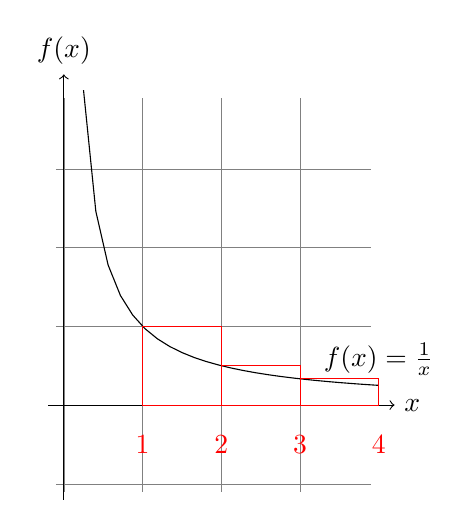
\begin{tikzpicture}[domain=0.25:4]
    \draw[very thin,color=gray] (-0.1,-1.1) grid (3.9,3.9);
    \draw[->] (-0.2,0) -- (4.2,0) node[right] {$x$};
    \draw[->] (0,-1.2) -- (0,4.2) node[above] {$f(x)$};
    \draw plot (\x,1/\x) node[above] {$f(x) =\frac{1}{x}$};
    \draw[color=red] (1,0) rectangle (2,1);
    \draw[color=red] (2,0) rectangle (3,0.5);
    \draw[color=red] (3,0) rectangle (4,0.333);
    \draw[color=red] (1,-0.5) node {$1$};
    \draw[color=red] (2,-0.5) node {$2$};
    \draw[color=red] (3,-0.5) node {$3$};
    \draw[color=red] (4,-0.5) node {$4$};
\end{tikzpicture}
The Left Riemann Sum is $>$ than $f(x)$:
\begin{align*}
    \frac{1}{1}+\frac{1}{2}+\frac{1}{3}+... 
    \Longrightarrow \sum_{n=1}^{\infty}{\frac{1}{n}} > \int_{1}^{\infty}{\frac{1}{x}}dx
\end{align*}
Similarly, \\
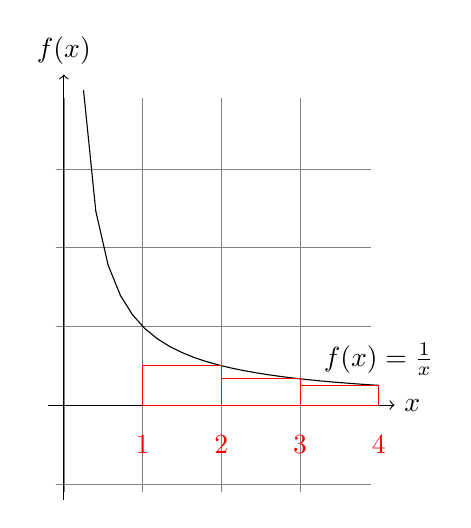
\begin{tikzpicture}[domain=0.25:4]
    \draw[very thin,color=gray] (-0.1,-1.1) grid (3.9,3.9);
    \draw[->] (-0.2,0) -- (4.2,0) node[right] {$x$};
    \draw[->] (0,-1.2) -- (0,4.2) node[above] {$f(x)$};
    \draw plot (\x,1/\x) node[above] {$f(x) =\frac{1}{x}$};
    \draw[color=red] (1,0) rectangle (2,0.5);
    \draw[color=red] (2,0) rectangle (3,0.3333);
    \draw[color=red] (3,0) rectangle (4,0.25);
    \draw[color=red] (1,-0.5) node {$1$};
    \draw[color=red] (2,-0.5) node {$2$};
    \draw[color=red] (3,-0.5) node {$3$};
    \draw[color=red] (4,-0.5) node {$4$};
\end{tikzpicture}
The Right Riemann Sum is $<$ than $f(x)$:
\begin{align*}
    \frac{1}{2}+\frac{1}{3}+\frac{1}{4}+... 
    \Longrightarrow \sum_{n=2}^{\infty}{\frac{1}{n}} < \int_{1}^{\infty}{\frac{1}{x}}dx \\
    \Longrightarrow \sum_{n=\textcolor{myred1}{1}}^{\infty}{\frac{1}{n}} < \int_{1}^{\infty}{\frac{1}{x}}dx + 1 \\
    \Longrightarrow \int_{1}^{\infty}{\frac{1}{x}}dx < \sum_{n=1}^{\infty}{\frac{1}{n}} < \int_{1}^{\infty}{\frac{1}{x}}dx + 1
\end{align*}

Using a method analogous to the Squeeze Theorem, if the bounds diverge, so does the series, and vice versa.

\section{P Series}
\textbf{NOT} Power Series. \\ 

A P Series is any series in the form:
$$
\sum_{n=0}^{\infty}{\frac{1}{n^p}}
$$
We use Integral Test to prove if it is diverging or converging.

\subsection{Harmonic Series}

A Harmonic Series is:
$$
\sum_{n=0}^{\infty}{\frac{1}{n}}
$$

Or a P Series where $p=1$.

\begin{align*}
    \int_{1}^{\infty}{\frac{1}{x}}dx < \sum_{n=1}^{\infty}{\frac{1}{n}} < \int_{1}^{\infty}{\frac{1}{x}}dx + 1
    \Longrightarrow \int_{1}^{\infty}{\frac{1}{x}}dx = \ln|x|\biggr\rvert^{\infty}_{1}
\end{align*}


\end{document}
